
%% bare_jrnl_comsoc.tex
%% V1.4b
%% 2015/08/26
%% by Michael Shell
%% see http://www.michaelshell.org/
%% for current contact information.
%%
%% This is a skeleton file demonstrating the use of IEEEtran.cls
%% (requires IEEEtran.cls version 1.8b or later) with an IEEE
%% Communications Society journal paper.
%%
%% Support sites:
%% http://www.michaelshell.org/tex/ieeetran/
%% http://www.ctan.org/pkg/ieeetran
%% and
%% http://www.ieee.org/

\documentclass[journal,comsoc]{IEEEtran}
%
% If IEEEtran.cls has not been installed into the LaTeX system files,
% manually specify the path to it like:
% \documentclass[journal,comsoc]{../sty/IEEEtran}


\usepackage[T1]{fontenc}% optional T1 font encoding






% *** CITATION PACKAGES ***
%
\usepackage{cite}

% cite.sty was written by Donald Arseneau
% V1.6 and later of IEEEtran pre-defines the format of the cite.sty package
% \cite{} output to follow that of the IEEE. Loading the cite package will
% result in citation numbers being automatically sorted and properly
% "compressed/ranged". e.g., [1], [9], [2], [7], [5], [6] without using
% cite.sty will become [1], [2], [5]--[7], [9] using cite.sty. cite.sty's
% \cite will automatically add leading space, if needed. Use cite.sty's
% noadjust option (cite.sty V3.8 and later) if you want to turn this off
% such as if a citation ever needs to be enclosed in parenthesis.
% cite.sty is already installed on most LaTeX systems. Be sure and use
% version 5.0 (2009-03-20) and later if using hyperref.sty.
% The latest version can be obtained at:
% http://www.ctan.org/pkg/cite
% The documentation is contained in the cite.sty file itself.





% *** GRAPHICS RELATED PACKAGES ***
\usepackage[pdftex]{graphicx}
\usepackage{epstopdf}

%
%\ifCLASSINFOpdf
%  \usepackage[pdftex]{graphicx}
%  % declare the path(s) where your graphic files are
%  % \graphicspath{{../pdf/}{../jpeg/}}
%  % and their extensions so you won't have to specify these with
%  % every instance of \includegraphics
%  % \DeclareGraphicsExtensions{.pdf,.jpeg,.png}
%\else
%  % or other class option (dvipsone, dvipdf, if not using dvips). graphicx
%  % will default to the driver specified in the system graphics.cfg if no
%  % driver is specified.
%  % \usepackage[dvips]{graphicx}
%  % declare the path(s) where your graphic files are
%  % \graphicspath{{../eps/}}
%  % and their extensions so you won't have to specify these with
%  % every instance of \includegraphics
%  % \DeclareGraphicsExtensions{.eps}
%\fi
% graphicx was written by David Carlisle and Sebastian Rahtz. It is
% required if you want graphics, photos, etc. graphicx.sty is already
% installed on most LaTeX systems. The latest version and documentation
% can be obtained at: 
% http://www.ctan.org/pkg/graphicx
% Another good source of documentation is "Using Imported Graphics in
% LaTeX2e" by Keith Reckdahl which can be found at:
% http://www.ctan.org/pkg/epslatex
%
% latex, and pdflatex in dvi mode, support graphics in encapsulated
% postscript (.eps) format. pdflatex in pdf mode supports graphics
% in .pdf, .jpeg, .png and .mps (metapost) formats. Users should ensure
% that all non-photo figures use a vector format (.eps, .pdf, .mps) and
% not a bitmapped formats (.jpeg, .png). The IEEE frowns on bitmapped formats
% which can result in "jaggedy"/blurry rendering of lines and letters as
% well as large increases in file sizes.
%
% You can find documentation about the pdfTeX application at:
% http://www.tug.org/applications/pdftex





% *** MATH PACKAGES ***
%
\usepackage{amsmath}

%\usepackage{bm}
% The bm.sty package was written by David Carlisle and Frank Mittelbach.
% This package provides a \bm{} to produce bold math symbols.
% http://www.ctan.org/pkg/bm





% *** SPECIALIZED LIST PACKAGES ***
%
%\usepackage{algorithmic}
% algorithmic.sty was written by Peter Williams and Rogerio Brito.
% This package provides an algorithmic environment fo describing algorithms.
% You can use the algorithmic environment in-text or within a figure
% environment to provide for a floating algorithm. Do NOT use the algorithm
% floating environment provided by algorithm.sty (by the same authors) or
% algorithm2e.sty (by Christophe Fiorio) as the IEEE does not use dedicated
% algorithm float types and packages that provide these will not provide
% correct IEEE style captions. The latest version and documentation of
% algorithmic.sty can be obtained at:
% http://www.ctan.org/pkg/algorithms
% Also of interest may be the (relatively newer and more customizable)
% algorithmicx.sty package by Szasz Janos:
% http://www.ctan.org/pkg/algorithmicx




% *** ALIGNMENT PACKAGES ***
%
%\usepackage{array}
% Frank Mittelbach's and David Carlisle's array.sty patches and improves
% the standard LaTeX2e array and tabular environments to provide better
% appearance and additional user controls. As the default LaTeX2e table
% generation code is lacking to the point of almost being broken with
% respect to the quality of the end results, all users are strongly
% advised to use an enhanced (at the very least that provided by array.sty)
% set of table tools. array.sty is already installed on most systems. The
% latest version and documentation can be obtained at:
% http://www.ctan.org/pkg/array


% IEEEtran contains the IEEEeqnarray family of commands that can be used to
% generate multiline equations as well as matrices, tables, etc., of high
% quality.




% *** SUBFIGURE PACKAGES ***
\usepackage[caption=false,font=footnotesize]{subfig}
%\ifCLASSOPTIONcompsoc
%  \usepackage[caption=false,font=normalsize,labelfont=sf,textfont=sf]{subfig}
%\else
%  \usepackage[caption=false,font=footnotesize]{subfig}
%\fi
% subfig.sty, written by Steven Douglas Cochran, is the modern replacement
% for subfigure.sty, the latter of which is no longer maintained and is
% incompatible with some LaTeX packages including fixltx2e. However,
% subfig.sty requires and automatically loads Axel Sommerfeldt's caption.sty
% which will override IEEEtran.cls' handling of captions and this will result
% in non-IEEE style figure/table captions. To prevent this problem, be sure
% and invoke subfig.sty's "caption=false" package option (available since
% subfig.sty version 1.3, 2005/06/28) as this is will preserve IEEEtran.cls
% handling of captions.
% Note that the Computer Society format requires a larger sans serif font
% than the serif footnote size font used in traditional IEEE formatting
% and thus the need to invoke different subfig.sty package options depending
% on whether compsoc mode has been enabled.
%
% The latest version and documentation of subfig.sty can be obtained at:
% http://www.ctan.org/pkg/subfig




% *** FLOAT PACKAGES ***
%
%\usepackage{fixltx2e}
% fixltx2e, the successor to the earlier fix2col.sty, was written by
% Frank Mittelbach and David Carlisle. This package corrects a few problems
% in the LaTeX2e kernel, the most notable of which is that in current
% LaTeX2e releases, the ordering of single and double column floats is not
% guaranteed to be preserved. Thus, an unpatched LaTeX2e can allow a
% single column figure to be placed prior to an earlier double column
% figure.
% Be aware that LaTeX2e kernels dated 2015 and later have fixltx2e.sty's
% corrections already built into the system in which case a warning will
% be issued if an attempt is made to load fixltx2e.sty as it is no longer
% needed.
% The latest version and documentation can be found at:
% http://www.ctan.org/pkg/fixltx2e


%\usepackage{stfloats}
% stfloats.sty was written by Sigitas Tolusis. This package gives LaTeX2e
% the ability to do double column floats at the bottom of the page as well
% as the top. (e.g., "\begin{figure*}[!b]" is not normally possible in
% LaTeX2e). It also provides a command:
%\fnbelowfloat
% to enable the placement of footnotes below bottom floats (the standard
% LaTeX2e kernel puts them above bottom floats). This is an invasive package
% which rewrites many portions of the LaTeX2e float routines. It may not work
% with other packages that modify the LaTeX2e float routines. The latest
% version and documentation can be obtained at:
% http://www.ctan.org/pkg/stfloats
% Do not use the stfloats baselinefloat ability as the IEEE does not allow
% \baselineskip to stretch. Authors submitting work to the IEEE should note
% that the IEEE rarely uses double column equations and that authors should try
% to avoid such use. Do not be tempted to use the cuted.sty or midfloat.sty
% packages (also by Sigitas Tolusis) as the IEEE does not format its papers in
% such ways.
% Do not attempt to use stfloats with fixltx2e as they are incompatible.
% Instead, use Morten Hogholm'a dblfloatfix which combines the features
% of both fixltx2e and stfloats:
%
% \usepackage{dblfloatfix}
% The latest version can be found at:
% http://www.ctan.org/pkg/dblfloatfix




%\ifCLASSOPTIONcaptionsoff
%  \usepackage[nomarkers]{endfloat}
% \let\MYoriglatexcaption\caption
% \renewcommand{\caption}[2][\relax]{\MYoriglatexcaption[#2]{#2}}
%\fi
% endfloat.sty was written by James Darrell McCauley, Jeff Goldberg and 
% Axel Sommerfeldt. This package may be useful when used in conjunction with 
% IEEEtran.cls'  captionsoff option. Some IEEE journals/societies require that
% submissions have lists of figures/tables at the end of the paper and that
% figures/tables without any captions are placed on a page by themselves at
% the end of the document. If needed, the draftcls IEEEtran class option or
% \CLASSINPUTbaselinestretch interface can be used to increase the line
% spacing as well. Be sure and use the nomarkers option of endfloat to
% prevent endfloat from "marking" where the figures would have been placed
% in the text. The two hack lines of code above are a slight modification of
% that suggested by in the endfloat docs (section 8.4.1) to ensure that
% the full captions always appear in the list of figures/tables - even if
% the user used the short optional argument of \caption[]{}.
% IEEE papers do not typically make use of \caption[]'s optional argument,
% so this should not be an issue. A similar trick can be used to disable
% captions of packages such as subfig.sty that lack options to turn off
% the subcaptions:
% For subfig.sty:
% \let\MYorigsubfloat\subfloat
% \renewcommand{\subfloat}[2][\relax]{\MYorigsubfloat[]{#2}}
% However, the above trick will not work if both optional arguments of
% the \subfloat command are used. Furthermore, there needs to be a
% description of each subfigure *somewhere* and endfloat does not add
% subfigure captions to its list of figures. Thus, the best approach is to
% avoid the use of subfigure captions (many IEEE journals avoid them anyway)
% and instead reference/explain all the subfigures within the main caption.
% The latest version of endfloat.sty and its documentation can obtained at:
% http://www.ctan.org/pkg/endfloat
%
% The IEEEtran \ifCLASSOPTIONcaptionsoff conditional can also be used
% later in the document, say, to conditionally put the References on a 
% page by themselves.




% *** PDF, URL AND HYPERLINK PACKAGES ***
%
%\usepackage{url}
% url.sty was written by Donald Arseneau. It provides better support for
% handling and breaking URLs. url.sty is already installed on most LaTeX
% systems. The latest version and documentation can be obtained at:
% http://www.ctan.org/pkg/url
% Basically, \url{my_url_here}.




% *** Do not adjust lengths that control margins, column widths, etc. ***
% *** Do not use packages that alter fonts (such as pslatex).         ***
% There should be no need to do such things with IEEEtran.cls V1.6 and later.
% (Unless specifically asked to do so by the journal or conference you plan
% to submit to, of course. )



% HB extensions ==V====v20150211=============================================
% HB Specific
\newcommand{\hbAverage}[1]{\overline{#1}}

% ======= HB ===============
% HB helper
\newcommand{\etal}{et al. }
\newcommand{\hbie}{i.e.,}
\newcommand{\hbeg}{e.g.,}


\newcommand{\hbSection}[1]{\section{#1}}
%\newcommand{\hbSection}[1]{}
%

\newcommand{\hbQuote}[1]{``\textsf{{\footnotesize #1}}''}
%\newcommand{\hbQuote}[1]{{\small \textsf{#1}}}
%\newcommand{\hbQuote}[1]{\textsf{#1}}
%{\footnotesize aaa}


%\newcommand{\hbIdea}[1]{}
\usepackage{color}
\newcommand{\hbIdea}[1]{{\color{red}{\scriptsize [{#1}]}}}

% HB picture size
%\newcommand{\myFigWidth}{.65\columnwidth}
\newcommand{\myFigWidth}{8cm}

% HB References
\usepackage[hidelinks]{hyperref} %boxes hidden, remove hidelinks if boxes are desired.
\newcommand{\reffig}[1]{Fig.~\ref{#1}}
\newcommand{\refeq}[1]{Eq.~\ref{#1}}
\newcommand{\reftbl}[1]{Table~\ref{#1}}
\newcommand{\refsec}[1]{Sec.~\ref{#1}}
\newcommand{\refthm}[1]{Theorem~\ref{#1}}
\newcommand{\refthmA}[2]{\refthm{#1}(\ref{#2}}
\newcommand{\reflem}[1]{Lemma~\ref{#1}}
\newcommand{\refdef}[1]{Definition~\ref{#1}}
\newcommand{\refexmp}[1]{Example~\ref{#1}}
\newcommand{\refitem}[1]{(\ref{#1})}
\newcommand{\refcite}[1]{ref~\cite{#1}}
% ======= HB ===============

%
%\usepackage[yyyymmdd,hhmmss]{datetime}

\usepackage[iso]{datetime}
\newcommand{\hbNow}{--Draft-- v\today/\currenttime} % version


%% HB Counter
%\newcounter{cntrObservation}
%\newcommand{\hCountDiff}{\stepcounter{cntrObservation}\textbf{Observation~\arabic{cntrObservation}.~}}
%% HB Logic
%\newcommand{\hDefinitionIFF}{\ensuremath{ \ \overset{\Delta}{\longleftrightarrow}} \ } % <-->
%\newcommand{\hSuchThat}{\;|\;}
%% HB enumerate
%\usepackage{enumitem}
%\newenvironment{hEnumerateRoman}
%{\begin{enumerate}[label=\roman*.,leftmargin=*,topsep=-10pt,partopsep=0pt,parsep=0pt,itemsep=0pt]}
%{\end{enumerate}}
%\newenvironment{hEnumerateAlpha}
%{\begin{enumerate}[label=\alph*) ,leftmargin=*,topsep=-10pt,partopsep=0pt,parsep=0pt,itemsep=0pt]}
%{\end{enumerate}}
% HB extensions ==A========================================================



% correct bad hyphenation here
\hyphenation{op-tical net-works semi-conduc-tor}


\begin{document}
%
% paper title
% Titles are generally capitalized except for words such as a, an, and, as,
% at, but, by, for, in, nor, of, on, or, the, to and up, which are usually
% not capitalized unless they are the first or last word of the title.
% Linebreaks \\ can be used within to get better formatting as desired.
% Do not put math or special symbols in the title.
\title{
%	Gender Compatibility in Selecting Partner
	Compatibility in Mate Selection
	{\small \\ \hbNow}  % <<<<<<<<<<<<<<<<<<<<<<<<<<<<<<<<<<<<<<<<<<
}
%
%
% author names and IEEE memberships
% note positions of commas and nonbreaking spaces ( ~ ) LaTeX will not break
% a structure at a ~ so this keeps an author's name from being broken across
% two lines.
% use \thanks{} to gain access to the first footnote area
% a separate \thanks must be used for each paragraph as LaTeX2e's \thanks
% was not built to handle multiple paragraphs
%

\author{Haluk~O.~Bingol,
        Omer~Basar% <-this % stops a space
\thanks{
H.~O.~Bingol  and Omer Basar are with 
the Department of Computer Engineering, 
Bogazici University, 
Istanbul,
34342 Turkey 
e-mail: bingol@boun.edu.tr.
}% <-this % stops a space
\thanks{Manuscript received December 1, 2015; revised XX XX, 2015.}}

% note the % following the last \IEEEmembership and also \thanks - 
% these prevent an unwanted space from occurring between the last author name
% and the end of the author line. i.e., if you had this:
% 
% \author{....lastname \thanks{...} \thanks{...} }
%                     ^------------^------------^----Do not want these spaces!
%
% a space would be appended to the last name and could cause every name on that
% line to be shifted left slightly. This is one of those "LaTeX things". For
% instance, "\textbf{A} \textbf{B}" will typeset as "A B" not "AB". To get
% "AB" then you have to do: "\textbf{A}\textbf{B}"
% \thanks is no different in this regard, so shield the last } of each \thanks
% that ends a line with a % and do not let a space in before the next \thanks.
% Spaces after \IEEEmembership other than the last one are OK (and needed) as
% you are supposed to have spaces between the names. For what it is worth,
% this is a minor point as most people would not even notice if the said evil
% space somehow managed to creep in.



% The paper headers
\markboth{Journal of \LaTeX\ Class Files,~Vol.~14, No.~8, August~2015}%
{Shell \MakeLowercase{\textit{et al.}}: Bare Demo of IEEEtran.cls for IEEE Communications Society Journals}
% The only time the second header will appear is for the odd numbered pages
% after the title page when using the twoside option.
% 
% *** Note that you probably will NOT want to include the author's ***
% *** name in the headers of peer review papers.                   ***
% You can use \ifCLASSOPTIONpeerreview for conditional compilation here if
% you desire.




% If you want to put a publisher's ID mark on the page you can do it like
% this:
%\IEEEpubid{0000--0000/00\$00.00~\copyright~2015 IEEE}
% Remember, if you use this you must call \IEEEpubidadjcol in the second
% column for its text to clear the IEEEpubid mark.



% use for special paper notices
%\IEEEspecialpapernotice{(Invited Paper)}




% make the title area
\maketitle

% As a general rule, do not put math, special symbols or citations
% in the abstract or keywords.
\begin{abstract}
	Mating is important for evolution.
	Since mating requires agreement of both parties, 
	although men and women have different preferences in partner selection, 
	there should be compatibility in these preferences. 
	How compatible are the preferences of male and female in a given property
	such as age, height, education and income?
	
	We have investigated the mating preferences 
	of females and males on a large online dating site.
	We use the most restricted definition of mating in our data
	which reduces the population size with \emph{N}~=~44,253.
	We confirm that females and males have different mating preferences.
	Females	prefer 
	taller and 
	older males with 
	better education and 
	higher income.
	Males prefer just the opposite.
	Our findings indicate that these differences complement each other
	in such a way that majority of the partners are happy with their mates.
\end{abstract}

% Note that keywords are not normally used for peerreview papers.
\begin{IEEEkeywords}
	Mating,
	mate selection,
	mating preferences,
	parental investment,
	gender compatibility,
	evolution,
	online dating.
\end{IEEEkeywords}






% For peer review papers, you can put extra information on the cover
% page as needed:
% \ifCLASSOPTIONpeerreview
% \begin{center} \bfseries EDICS Category: 3-BBND \end{center}
% \fi
%
% For peerreview papers, this IEEEtran command inserts a page break and
% creates the second title. It will be ignored for other modes.
\IEEEpeerreviewmaketitle



% 
%\section{Introduction}
% The very first letter is a 2 line initial drop letter followed
% by the rest of the first word in caps.
% 
% form to use if the first word consists of a single letter:
% \IEEEPARstart{A}{demo} file is ....
% 
% form to use if you need the single drop letter followed by
% normal text (unknown if ever used by the IEEE):
% \IEEEPARstart{A}{}demo file is ....
% 
% Some journals put the first two words in caps:
% \IEEEPARstart{T}{his demo} file is ....
% 
% Here we have the typical use of a "T" for an initial drop letter
% and "HIS" in caps to complete the first word.



% ========================================================================
\section{Introduction}

\hbIdea{gender differences} % ====================
\IEEEPARstart{T}{here} 
%There 
has been a long debate on how different male and female are~\cite{
	Darwin1871Book,
	Tannen1991Book,
	Buss2003Book,
	Gray2009Book,
	Liljeros2001Nature,
	Schmitt2008,
	CelaConde2009PNAS,
	Hyde2009PNAS,
	Szell2013SR,
	Blanch2015,
	Hyde2005,
	Zell2015}.
\emph{Gender difference hypothesis} claims that 
males and females are very different in their 
personalities,
abilities,
interests,
attitudes and 
behavioral tendencies~\cite{
	Tannen1991Book,
	Buss2003Book,
	Gray2009Book,
	Liljeros2001Nature,
	Schmitt2008,
	CelaConde2009PNAS,
	Hyde2009PNAS,
	Szell2013SR,
	Blanch2015}.
Some recent findings support this hypothesis.
Men and women are different in many ways including
sexual contacts~\cite{
	Liljeros2001Nature},
in brain imaging studies~\cite{
	CelaConde2009PNAS},
performance in Mathematics~\cite{
	Hyde2009PNAS}, 
or chess~\cite{
	Blanch2015},
even online games~\cite{
	Szell2013SR}.
On the other hand, 
some investigations support the \emph{gender similarity hypothesis} 
which claims that 
the difference is not as big as one expects~\cite{
	Hyde2005,
	Zell2015}.

\hbIdea{hunter-gatherer theory} % ====================
One possible evolutionary explanation of the gender difference is 
the \emph{hunter-gatherer theory of spatial sex differences} 
proposed by Silverman and Earl~\cite{
	Silverman1992}. 
It claims that there has been division of labor between men and women
as early as the time of hunter-gatherers.
Males are primarily hunters and females primarily foraged.
This affects the cognitive development since
\hbQuote{
	tracking and killing animals entail different kinds of spatial problems 
	than does foraging for edible plants; 
	thus,
	adaptation would have favored diverse spatial skills between sexes 
	throughout much of their evolutionary history
}.
Hence, 
it calls for different spatial skills such as
mental rotations,
map reading,
maze learning 
for male.
and
ability to learn, recognize, remember spatial configurations of objects,
and their spatial relationships 
for female.




% ========================================================================
\subsection{Mating and Parental Investment}

\hbIdea{mating and parental investment theory} % ====================
Mating is important for evolution.
%There are gender differences in mating, too. 
In many species, it has been observed that 
male and female have different strategies in mate 
selection.

We need an evolutionary theory 
to explain differences in mating strategies. 
One such theory is 
Trivers' 
\emph{parental investment theory} 
which is based on parental investment~\cite{
	Trivers1972}.
%An evolutionary theory 
%that explains differences in mating strategies 
%is \emph{parental investment theory} proposed by 
%Trivers~\cite{
%	Trivers1972}.
Offsprings, having support from parents, have better chance to survive, 
hence to reproduce.
Therefore, 
evolution calls for parental support.
He carefully defines \emph{parental investment} as
\hbQuote{
	any investment by the parent in an individual offspring 
	that increases the offspring's chance of surviving 
	(and hence reproductive success)
	at the cost of the parent's ability to invest in other offspring
}.

\hbIdea{mating strategies} % ====================
Parental investment is quite uneven between male and female
in many species~\cite{
	Trivers1972}.
Therefore both genders evolutionarily developed mating strategies 
which are clearly different~\cite{
	Buss1989,
	Buss1993,
	Buss2003Book,
	Buss2006}.
\hbIdea{female strategy} % ====================
In female mammal, 
hence human female, 
is forced to select quality,
since she cannot choose quantity.
Human female makes mandatory high investment in offspring compared to male,
if one considers nine months of gestation, childbirth, lactation, nurturing.
Therefore, 
she looks for supporting male in her mate selection.
She prefers a male who 
not only have the resources to support her 
but also willing to commit these resources to her.
That explains female preference for \emph{long-term} commitment.
\hbIdea{female strategy} % ====================
On the other hand, 
human male can choose quantity.
He is reluctant to long-term commitment. 
He has a tendency for \emph{short-term} relations
which increase his chances to reproduce offsprings.
This quality versus quantity paradigm is clearly a conflict 
that has to be resolved.
Female, 
who invest more in offspring,
should be more choosy selecting mate
(\emph{intersexual attractio}n)
and
male,
who invest less,
should compete to access the opposite sex
(\emph{intrasexual competition})~\cite{
	Trivers1972}.





% ========================================================================
\subsection{Properties in Mate Selection}

%How do you judge fertility or reproductive value?
%The only clue is the observations one can make.
%For example, 
%by evolution,
%male has learned to look for 
%(i)~physical features (\hbeg
%	symmetry,
%	good muscle tone,
%	absence of lesions),
%(ii)~observable behavior (\hbeg
%	sprightly,
%	high activity level),
%(iii)~social reputation (\hbeg
%	knowledge gathered from others)~\cite{
%	Buss1989,
%	Buss1993,
%	Buss2006}.
%
%By evolution, 
%Male looks for 
%full lips,
%smooth skin,
%lustrous hair,
%low ratio of hips to waist
%for fertility~\cite{
%	Buss1989,
%	Buss2006}.
%
%Female prefers male having properties such as 
%wealth, 
%masculine physical atributes
%such as 
%height,  


\hbIdea{mating properties} % ====================
Properties, 
that increase the chance of mating, 
become crucial in this respect~\cite{
	Buss1989,
	Buss1993,
	Buss2006,
	Trivers1972,
	Kenrick1992, % Male-older
	Gillis1980, % Male-taller
	Pawlowski2000Nature,  % Male-taller
	Swami2008,  % Male-taller
	Silverman1992,  % Male-taller
	Buss2003Book}.  % Male-taller
\hbIdea{age} % ====================
In terms of evolution,
% 
(a)~\emph{fertility},
\hbie~immidiate probability of conception,
and
%
(b)~\emph{reproductive value}
\hbie~future reproductive potential,
are the top two properties for both 
gender~\cite{
	Buss2006}.
	They are age related.
Clearly, health is also very important.
%the next property one looks for.
So young healthy mate should be the choice in all species.
Human male just does that.
But human female has other issues therefore being young is not enough.
She is looking for male that will provide parental support for her offspring,
that is,
he should 
%
(a)~have the resources and 
%
(b)~willingness to commit these resources to her offspring.
In order to collect resources he needs time.
Therefore he may not be that young after all.
\hbIdea{physical} % ====================
While female is busy providing parental investment to her offspring,
she expects male 
to provide food and shelter.
He is also expected to protect her and her offspring.
So physically masculine male should be preferred. 
\hbIdea{expect} % ====================
So we expect that younger female and 
``superior'' male partners.

Empirical evidences support these 
deductions~\cite{
	Schmitt2008,
	Buss1989,
	Buss2003Book,
	Kenrick1992, % Male-older
	Gillis1980, % Male-taller
	Pawlowski2000Nature,  % Male-taller
	Swami2008,  % Male-taller
	Silverman1992}.  % Male-taller
%Human male and female have different preferences in mate 
%selection~\cite{
%	Kenrick1992, % Male-older
%	Gillis1980, % Male-taller
%	Pawlowski2000Nature,  % Male-taller
%	Swami2008,  % Male-taller
%	Silverman1992,  % Male-taller
%	Buss2003Book}.  % Male-taller
Investigations on partners has revealed that
\hbIdea{age} % ====================
male is older~\cite{
	Kenrick1992},
\hbIdea{physical} % ====================
taller~\cite{
	Gillis1980,
	Pawlowski2000Nature,
	Swami2008}
than female.
This is a universal pattern across cultures~\cite{
	Buss1989,
	Schmitt2008}.




%% =========================================================================
%\subsection{Online Dating}
	


%Data
%that have never been reachable 
%before is available on internet~\cite{
%	Szell2010PNAS,
%	Centola2010Science,
%	Rocha2010PNAS,
%	Szell2013SR,
%	Kramer2014PNAS}.
%\hbIdea{ODS} % ====================
%Online dating cannot be kept away from this 
%trend~\cite{
%	Barraket2008JSociology,
%	Bingol2012PartnerArxiv,
%	Norcie2013LNCS,
%	Zhao2014IS}.




%% ========================================================================
%\subsection{Compatibility of Preferences}

\hbIdea{Compatibility of Preferences} % ====================
Since mating requires agreement of both parties, 
although men and women have different preferences in mate selection, 
there should be compatibility in these preferences. 
We can ask the following question.
How compatible are the preferences of two genders in a given property?

We will use the data obtained from an online dating site.
First we carefully define mating in our data set.
Then we aggregate the properties of partners that an individual selects as mate.
Finally we search for patterns in the properties for mating behavior.

%
%One such cross cultural study is done by 
%Buss~\cite{
%	Buss1989}.
%They investigate human mate preferences in 37 cultures with  
%4,601 male, 5,446 female, in total 10,047, 
%participants. 
%Participants are asked a series of questions about their preferences in selection of a mate.
%One of the questions is 
%the age difference they prefer to have.
%On the average,
%males prefer 2.66 years younger, 
%females prefer 3.42 years older mate than themselves.
%Note that this is just a desire which may not be realized
%due to many factors including local availability of mates, sex ratio.
%In the same study, based on another source,
%it is estimated that the average actual age difference of married couples is 2.99 years 
%which is close to the average of 2.66 and 3.42.
%Participants are also asked to rate given a set of characteristics 
%in the order of importance in choosing a mate.
%%The rating scale ranges from 
%%3 (indispensable) to 
%%0 (irrelevant or unimportant).
%Among those characteristics, 
%``good financial prospects'' is related to our study.
%They observed that, 
%except Spain, 
%in all 36 countries females value 
%``good financial prospects'' significantly more than males.




% =========================================================================
\section{Method}




% =========================================================================
\subsection{Data Set}
	

\hbIdea{online dating data} % ====================
We investigate the data of a large Turkish online dating site 
for compatibility of mating preferences~\cite{
	Bingol2012PartnerArxiv}.
There are 4,500,000 registered users in total.
More than 3,000 new users register daily. 
A user stay in the system for 3 months, on the average. 
Many of them come back, later;
sometimes as a new user.
The daily activity is also quite large such as 
50,000 user logins,
500,000 massage transactions, 
5,000 photo uploads, and 
20,000 votes.




% =========================================================================
\subsection{Definition of Mating}

\hbIdea{online dating} % ====================
A typical online dating system enables its user to 
find partner that best matches one's desires.
Each user defines his user profile.
An initiator, predominantly male, 
selects a potential partner by examining her profile and 
sends her a message.
If there is a positive response from the receiver, 
then more messages are exchanged
which hopefully leads to a face-to-face meeting.

\hbIdea{partner criteria} % ====================
When do we say that male and female are mating?
Online dating site has lots of information about the virtual world, 
but there is usually no information whether 
the male and the female really make a mating partner in the physical world.
Any action in an online dating site is clearly an attempt for mating
but is it sufficient to be considered as mating?
For example,
%(i)~
just sending a message,
%(ii)~
getting a message in response, 
or 
%(iii)~
some more exchange of messages 
should not be enough in the world of online dating which is full of these.
%make them a partner.

%Usually online dating sites do not have any information 
%whether 
%the male and the female really make a partner in the physical world.
Therefore we select  
the most restricted criteria of mutual interest, 
that is available in our data set,
which is virtual gifts~\cite{Bingol2012PartnerArxiv}.
Receiving a \emph{virtual gift}, 
which is usually a picture of a flower, 
is considered  a ``value'' in this virtual society.
We have even observed that some user sent virtual gifts to themselves.
This value is probably due to
(i)~the virtual gifts one receives is visible to all,
(ii)~they are not free, 
\hbie\ one has to purchase virtual gifts in order to sent, and
(iii)~only qualified users can sent virtual gifts.
Since unpaid male members are not qualified to sent gifts, 
able to sent gifts may be considered as an indication of wealth.

There are $276,210$ male and 
$483,963$ female users that are qualified to send virtual gift in the system. 
Among those, only 
$29,274$ male and 
$14,981$ female,
in total $N = 44,253$, 
users reciprocally exchange virtual gifts.
Hence we define a pair as (mating) \emph{partners} if
they not only exchange messages, 
but also 
send at least one gift to, 
and 
receive at least one gift from each other.

Note that  
this definition is based on actual behaviors of users in the online dating site.
We have the ``actual'' partners,
that is,
they mutually agree to ``mate'' 
as far as we can trace in our online dating site, 
rather than 
a ``theoretical'' partner one wishes to have 
as he answers the questions of a survey
as in the case of \refcite{
	Buss1989}.
We have such theoretical data in user profiles, too. 
Users specify what properties, 
such as the age, height, 
they look for in their potential partners.
This data is noisy.
Users are not consistent.
They claim something and does something else.
For example,
someone claims that he prefers women taller than 170~cm but
does not hesitate to be partner with a 160~cm.
Such behavior is clearly difficult to register in questionaries.
In this respect our actual data deserves special attention.

	




% =========================================================================
\subsection{Properties of the Mate}

\hbIdea{properties of the mate} % ====================
Once we have identified the partners,
we investigate the properties of the mate.
As expected, 
user $i$ becomes partner with many others as time goes.
Each partner of $i$ may have different value for property $p$.
The average of the properties of the partners of $i$ 
is given as
\[
	\hbAverage{p_{i}} = \frac{1}{|C_{i}|}  \sum_{j \in C_{i}} p_{j}
\]
where 
$p_{j}$ denotes the property $p$ as it is defined in user $j$'s profile
and 
$C_{i}$ is the set of users that $i$ partnered with.
We interpret this as
user $i$ has a tendency to select partners having value of 
$\hbAverage{p_{i}}$ in property $p$ .
%That is,
%$i$ \emph{prefers} $\hbAverage{p_{i}}$ in her partners.
Hence, 
we call $\hbAverage{p_{i}}$ as the \emph{preferred value} for $i$.
%
Instead of using the preferred value directly,
we compare one's own value
to the preferred value that one looks in his partners.
The \emph{preferred difference} of $i$, 
in property $p$, 
is defined as
%\begin{linenomath*}
\[
	\Delta p_{i} = p_{i} - \hbAverage{p_{i}}.
\]
%\end{linenomath*}
Note that $\Delta p_{i}$ can be negative or positive. 
If $\Delta p_{i}$ is around $0$
then the user prefers partners with similar properties with him, 
i.e. homophily~\cite{
	McPherson2001,
	Centola2011Science}.
For example, 
if the property is height
and
if user $i$ has a tendency for taller partner in her selection,
then $\Delta p_{i}$ would be negative.




% =========================================================================
\subsection{Distribution of Preferred Differences}

\hbIdea{property distribution} % ====================
We can extend these concepts from individual $i$ to a group of people.
Then, frequency of people with the same preferred difference 
makes a probability distribution,
which we call \emph{preferred difference distribution}.
Having 
all women as one group, and 
all men as another group,
we obtain two preferred difference distributions
$f(x)$ and $m(x)$ of females and males, respectively. 




% =========================================================================
\section{Results}

\hbIdea{findings} % ====================
The statistical parameters of the preferred differences in 
age, height, education and income are given in
\reftbl{tbl:statistics}.
Columns 
$\mu_{m}$,  $\mu_{f}$, 
and
$\sigma_{m}$, $\sigma_{f}$ are the
averages and standard deviations of males and females, respectively.
The distributions of the preferred differences
%for 
%height, age, education and income 
are given in  \reffig{fig:propertyDifference}.
We first focus on the averages,
and leave the discussion of 
distributions and 
their compatibility, 
the last column of \reftbl{tbl:statistics}, 
later.




% =========================================================================
\subsection{Average of Preferred Differences}

In all four properties in \reftbl{tbl:statistics},
there is a distinct pattern.
The averaged preferred differences 
for males, $\mu_{m}$, are all negative 
and
that of females are all positive. 
This observation indicates that in all four properties, 
whatever the metric is used to measure the property,
males prefer ``inferior'' females
and females prefer ``superior'' males compared to themselves.


\hbIdea{age} % ====================
\textbf{Age.}
According to evolutionary theories,
we expect to see younger female and older male in partners.
Our findings confirms that.
We observe that,
on the average, 
males mate with females $2.90$ years younger than themselves,
and
females mate with males $2.74$ years older.
Our findings are in agreement with 
males prefer 2.66 years younger, 
females prefer 3.42 years older mate than themselves reported by Buss~\cite{
	Buss1989}.
%
%In a comparable cross cultural study ($N = 10,047$),
%Buss reports that, 
%on the average,
%males prefer 2.66 years younger, 
%females prefer 3.42 years older mate than themselves~\cite{
%	Buss1989}.
%Our findings in agreement with this.



%They investigate human mate preferences in 37 cultures with  
%4,601 male, 5,446 female, in total $N = 10,047$, 
%participants. 
%Participants are asked a series of questions about their preferences in selection of a mate.
%It is reported that,

%
%One such cross cultural study is done by 
%Buss~\cite{
%	Buss1989}.
%They investigate human mate preferences in 37 cultures with  
%4,601 male, 5,446 female, in total 10,047, 
%participants. 
%Participants are asked a series of questions about their preferences in selection of a mate.
%One of the questions is 
%the age difference they prefer to have.
%On the average,
%males prefer 2.66 years younger, 
%females prefer 3.42 years older mate than themselves.
%Note that this is just a desire which may not be realized
%due to many factors including local availability of mates, sex ratio.
%In the same study, based on another source,
%it is estimated that the average actual age difference of married couples is 2.99 years 
%which is close to the average of 2.66 and 3.42.

%	Participants are also asked to rate given a set of characteristics 
%	in the order of importance in choosing a mate.
%	%The rating scale ranges from 
%	%3 (indispensable) to 
%	%0 (irrelevant or unimportant).
%	Among those characteristics, 
%	``good financial prospects'' is related to our study.
%	They observed that, 
%	except Spain, 
%	in all 36 countries females value 
%	``good financial prospects'' significantly more than males.
%	====

%The average preferred difference in age is 
%$-2.90$ and $2.74$ years for males and females, respectively.
%Considering the extreme values 
%$-7.38$ (Zambian males ) and $5.10$ (Iranian females) years,
%the averages
%$-2.66$ for male and $3.42$ for female  
%of \refcite{Buss1989}
%are in agreement with our figures.
%One observation is that male and female averages close to different countries.
%For males, 
%the countries close to $-2.90$ are 
%	Poland ($-2.85$),
%	Israel (Jewish) ($-2.88$),
%	Brazil ($-2.94$), and
%	Venezuela ($-2.99$).
%For females,
%close to $2.74$ are
%	Canada (English) ($2.72$),
%	Netherlands ($2.72$),
%	Ireland ($2.78$), and
%	Finland ($2.83$).
%
%The statistical parameters 
%$\mu_{m}$,  $\mu_{f}$, 
%and
%$\sigma_{m}$, $\sigma_{f}$ of preferred difference distributions of genders
%are given in \reftbl{tbl:statistics}.








\hbIdea{difference in partner selection} % ====================
\textbf{Height.}
Our findings on preferred difference in height, given in \reffig{fig:propertyDifferenceHeight}, agree with the previous work.
People usually interact with people who have similar 
characteristics~\cite{
	McPherson2001,
	Centola2011Science}.
For example 
no drastic height differences between partners are observed.
That is, 
tall male partners with tall female, and short with 
short~\cite{
	Gillis1980,
	Swami2008}.
Although there are males prefer females 
$30$\,cm shorter
or 
$10$\,cm taller 
in \reffig{fig:propertyDifferenceHeight},
they are rare.
%This is a manifestation of homophily in height.
%tall men partners with tall women.
Majority are accumulated around the average
which is a
manifestation of homophily in height.

Yet, 
there are distinct differences between the preferences of male and female
%This is not exactly the case for partner selection.
%Different genders have different preferences in properties 
when it comes to partner selection,
such as height~\cite{
	Gillis1980,
	Swami2008,
	Pawlowski2000Nature}.
Male is usually taller then female in partners,
which is called \emph{male-taller norm}~\cite{
	Gillis1980}.
The averages in \reftbl{tbl:statistics}
agree with the male-taller norm.
On the average, 
male prefers female 
$11.12$\,cm shorter.
Similarly, 
on the average
females prefer male 
$11.37$\,cm taller.

\textbf{Income and Education.}
We observe similar pattern in income and education, too,
namely,
males prefer negative and females prefer positive differences.
Here the numbers cannot be compared with other works directly
since 
users are asked to select one bin out of many bins 
which are organized in a consistent but an arbitrary way. 
They are consistent in the sense that the larger the bin number,
the more educated or higher income.
The bins in education are related to the number of schooling years
such as
graduate of primary school, or
of college.
The bins in income field represent monthly income such as 
bin 2: $500 < x < 1000$,
bin 3: $1000 < x < 2000$.

%Both income and education are selected from
%For example,
%for the income field of data, 
%user is allow to select one out of five income bins, namely, 
%bin 1: $x < 500$, 
%bin 2: $500 < x < 1000$,
%bin 3: $1000 < x < 2000$,
%bin 4: $2000 < x < 3000$, and 
%bin 5: $3000 < x$. 
%So what we can do is to compare the bins of the partners.


% =========================================================================
% TABLE HERE 
% {tbl:statistics}
% -------------------------------------------------------------------------
\begin{table}%[htdp]
\caption{Comparison of male and female distributions}
\begin{center}
%\begin{tabular*}{\hsize}{@{\extracolsep{\fill}}|l|rr|rr|c|}
\begin{tabular*}{\hsize}{@{\extracolsep{\fill}}lrrrrc}
% -------------------------------
\hline
Property
&\multicolumn{2}{c}{Averages}
&\multicolumn{2}{c}{Standard Deviations}
&Compatibility\\
% 
&$\mu_{m}$
&$\mu_{f}$
&$\sigma_{m}$
&$\sigma_{f}$
&$\rho$\\
%
\hline
%
Height (cm)		
&-11.12 
&11.37 
&6.76
&7.09
&0.90\\
%
Education (bin)
&-0.36
&0.34
&1.35
&1.40
&0.92\\
%
Age (year)			
&-2.90
&2.74
&5.06
&5.23
&0.94\\
%
Income (bin)
&-0.93
&0.99
&1.28
&1.32
&0.95\\
\hline
% -------------------------------
\end{tabular*}
\end{center}
\label{tbl:statistics}
\end{table}
% -------------------------------------------------------------------------
% =========================================================================



% =========================================================================
% FIG HERE 
% {fig:propertyDifference}
% ------------------------------------------------------------------------
%\begin{figure}[ht]
\begin{figure*}%[ht]
\centering
%\begin{center}
	%
	\subfloat[Height]{
%		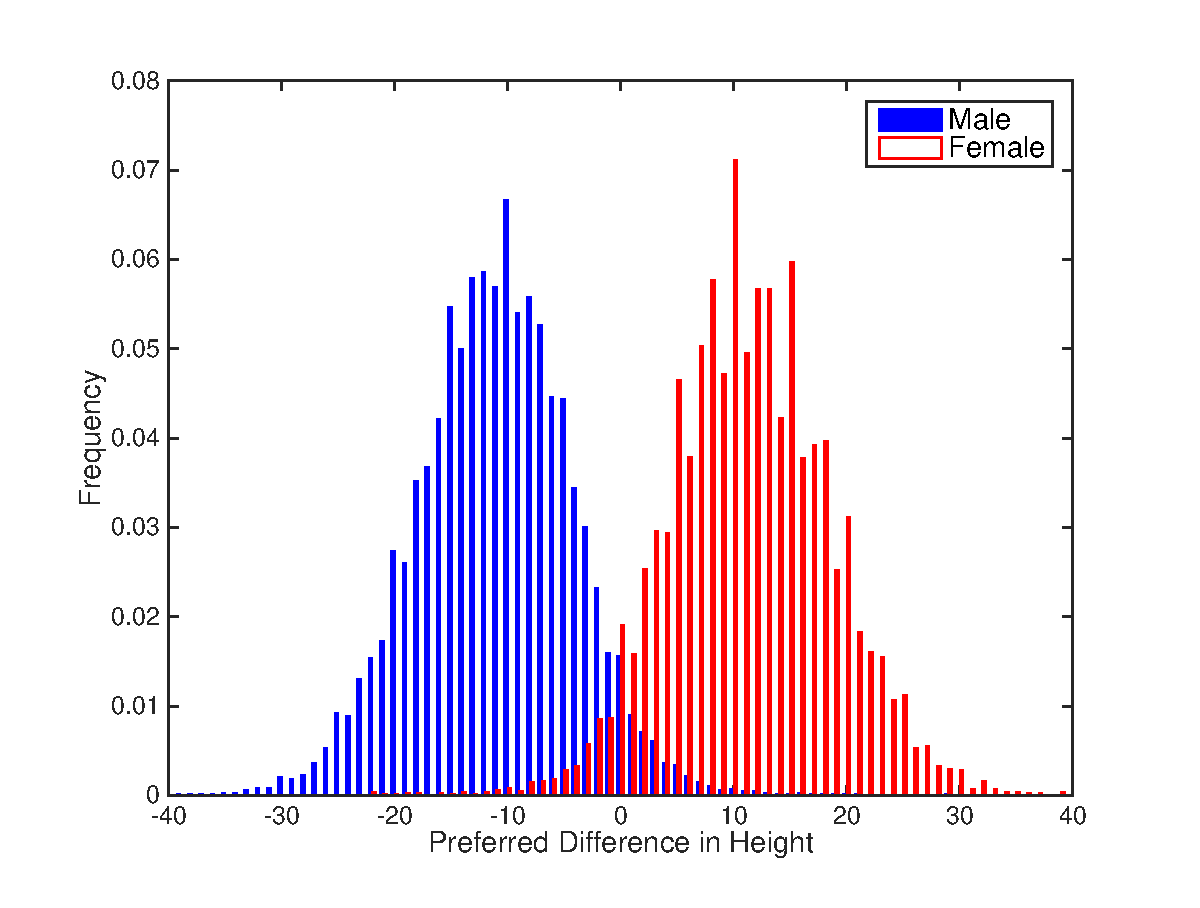
\includegraphics[width=.65\columnwidth]{imgDiff_Height}
		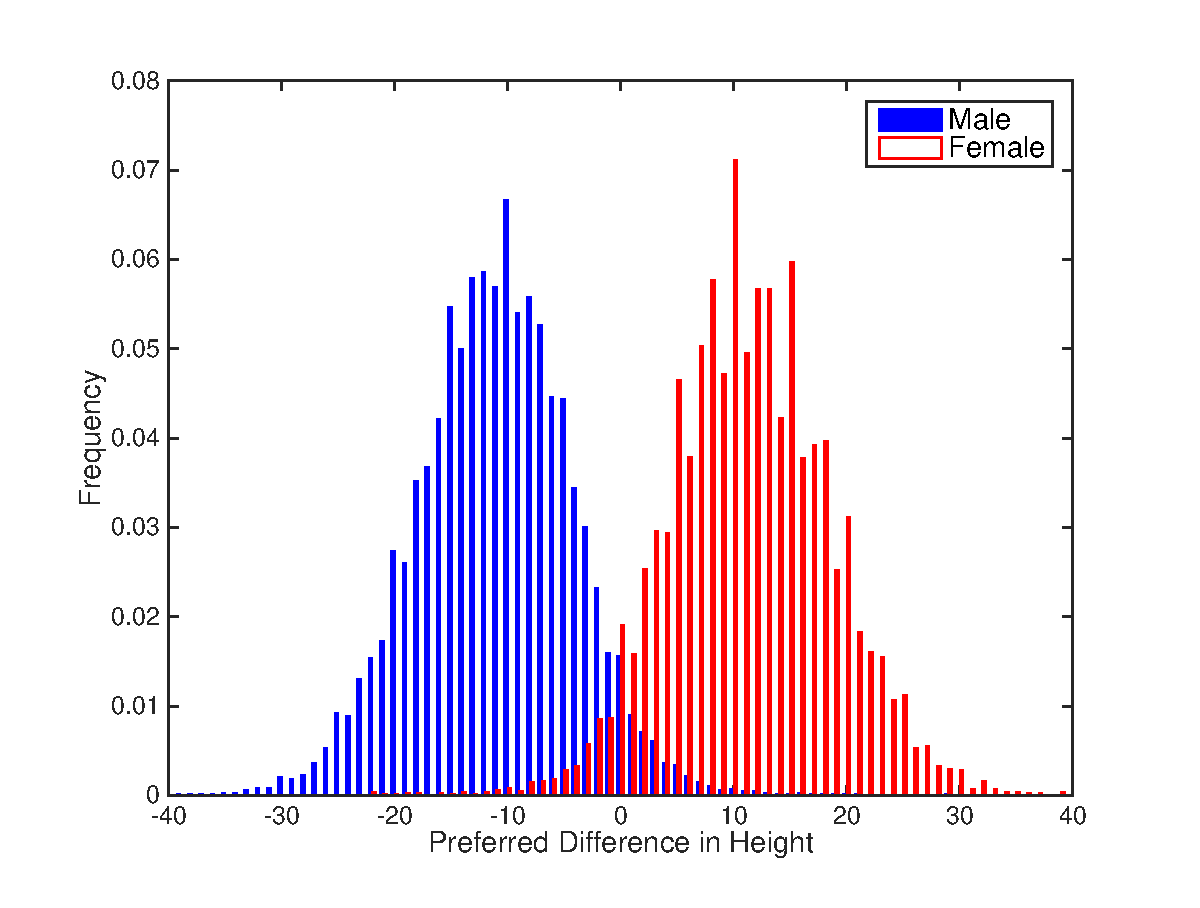
\includegraphics[width=\myFigWidth]{imgDiff_Height}
		\label{fig:propertyDifferenceHeight}
	}
	%
	\hfil
	\subfloat[Age]{
		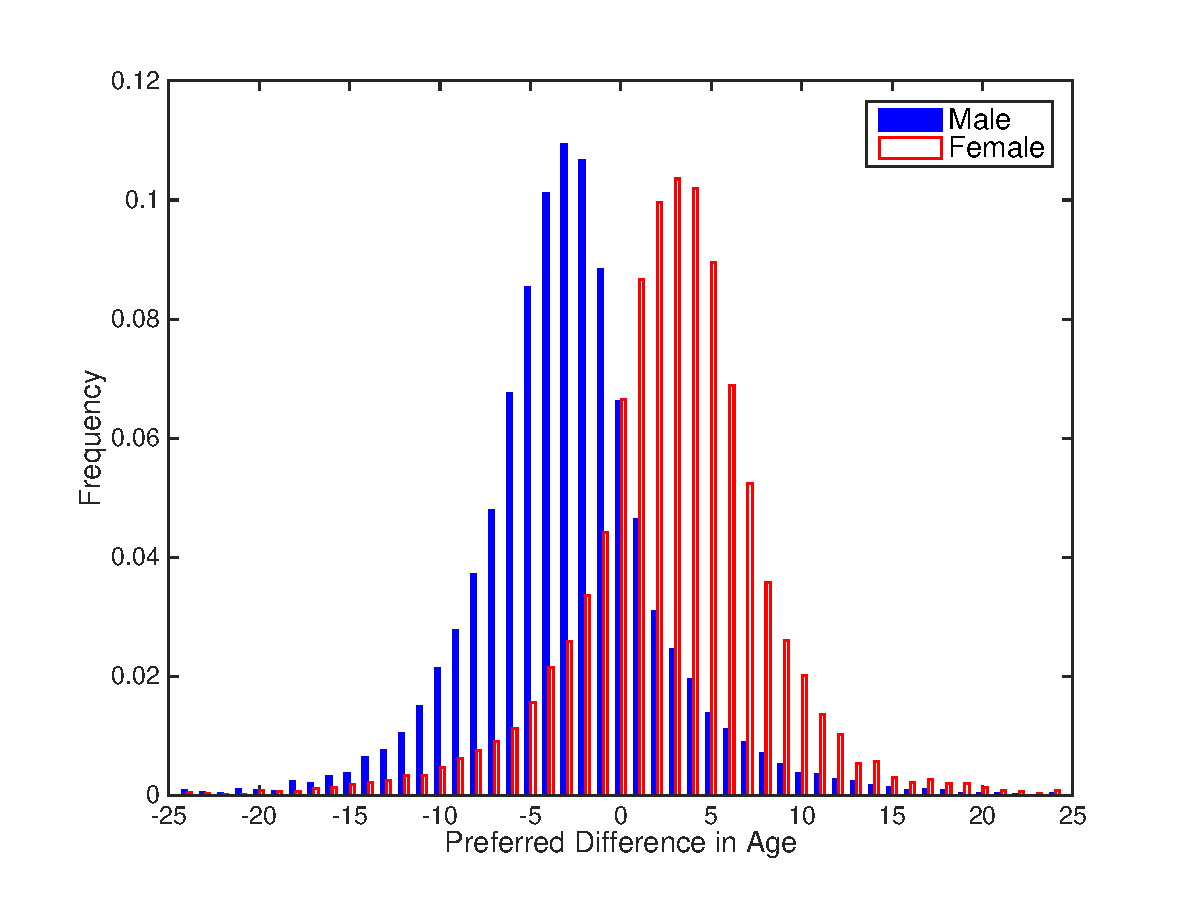
\includegraphics[width=\myFigWidth]{imgDiff_Age}
		\label{fig:propertyDifferenceAge}
	}\\
	%
%	\hfil
	\subfloat[Education]{
		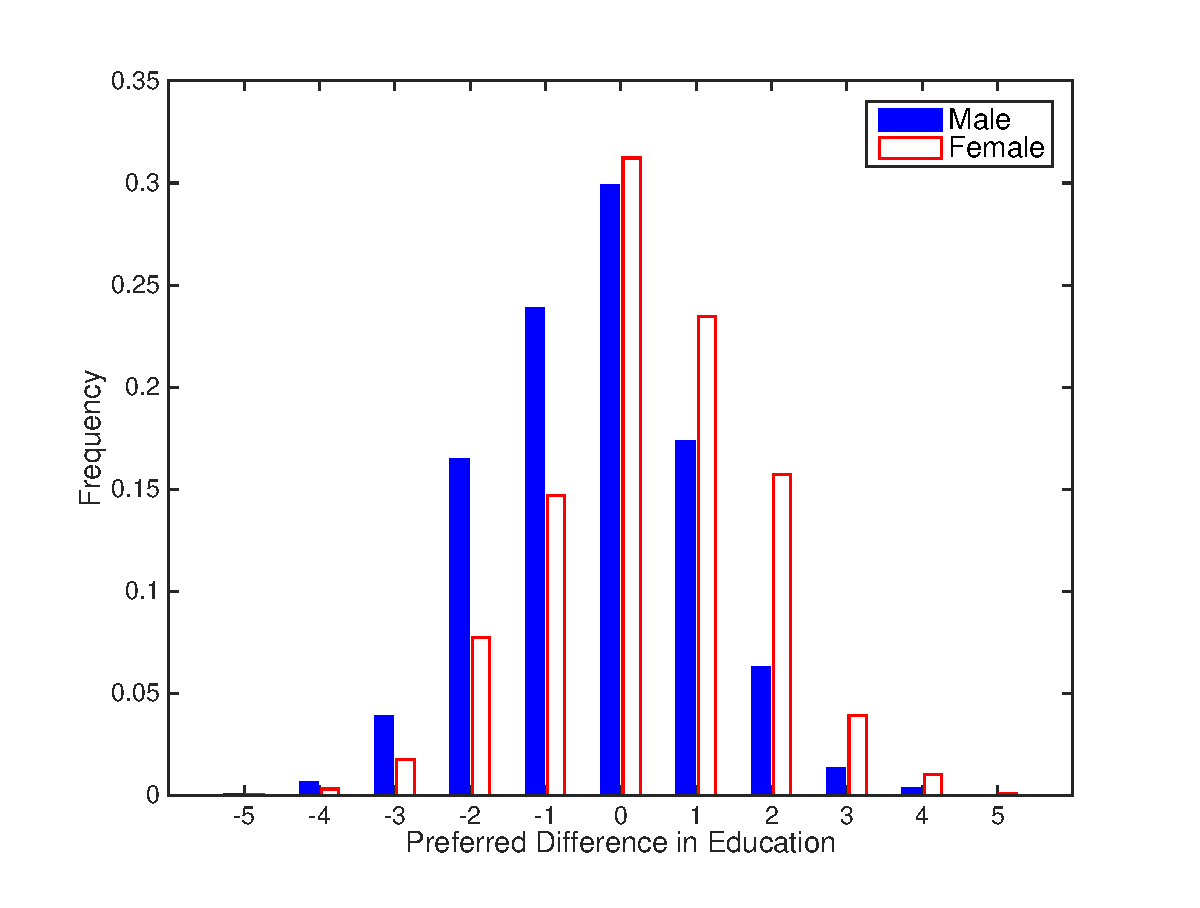
\includegraphics[width=\myFigWidth]{imgDiff_Education}
		\label{fig:propertyDifferenceEducation}
	}
	%
	\hfil
	\subfloat[Income]{
		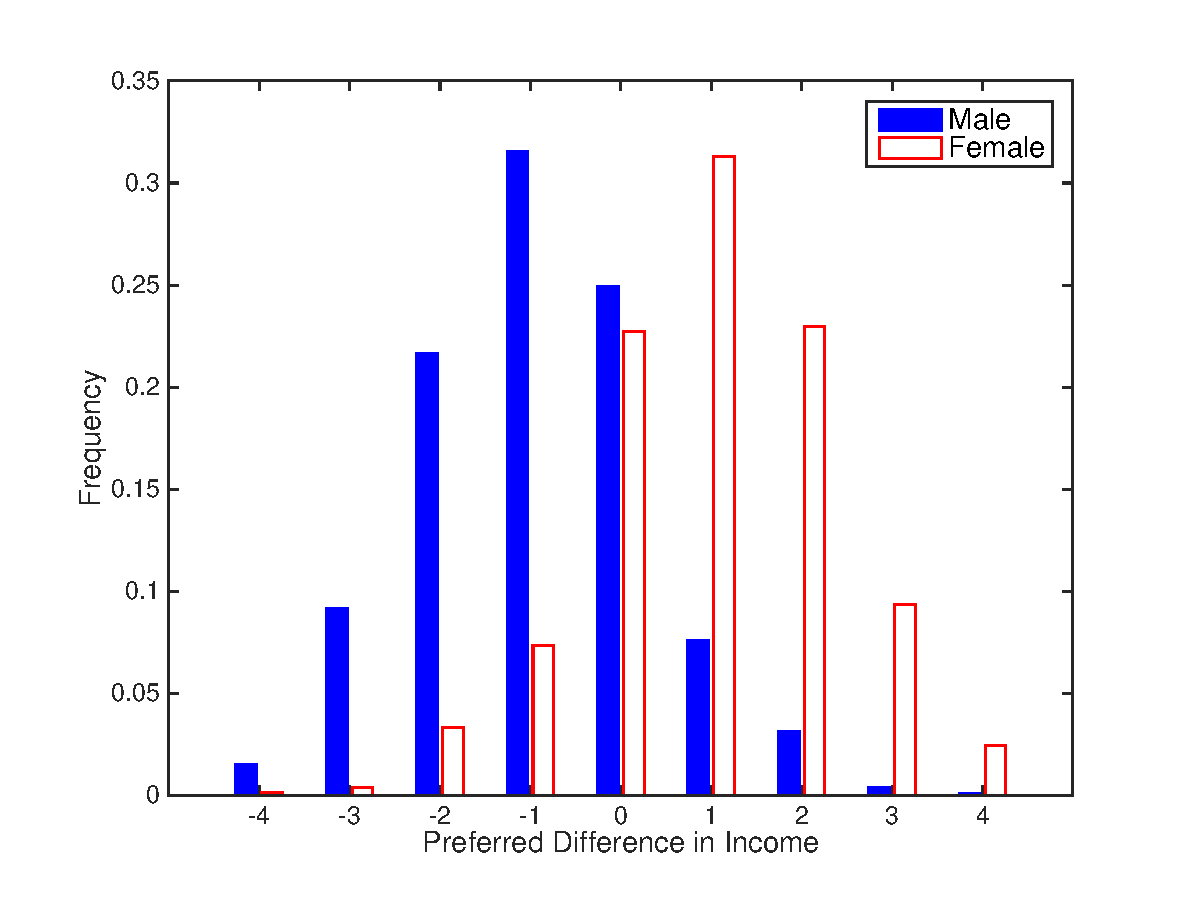
\includegraphics[width=\myFigWidth]{imgDiff_Income}
		\label{fig:propertyDifferenceSalary}
	}
%	\subfloat[BMI]{
%		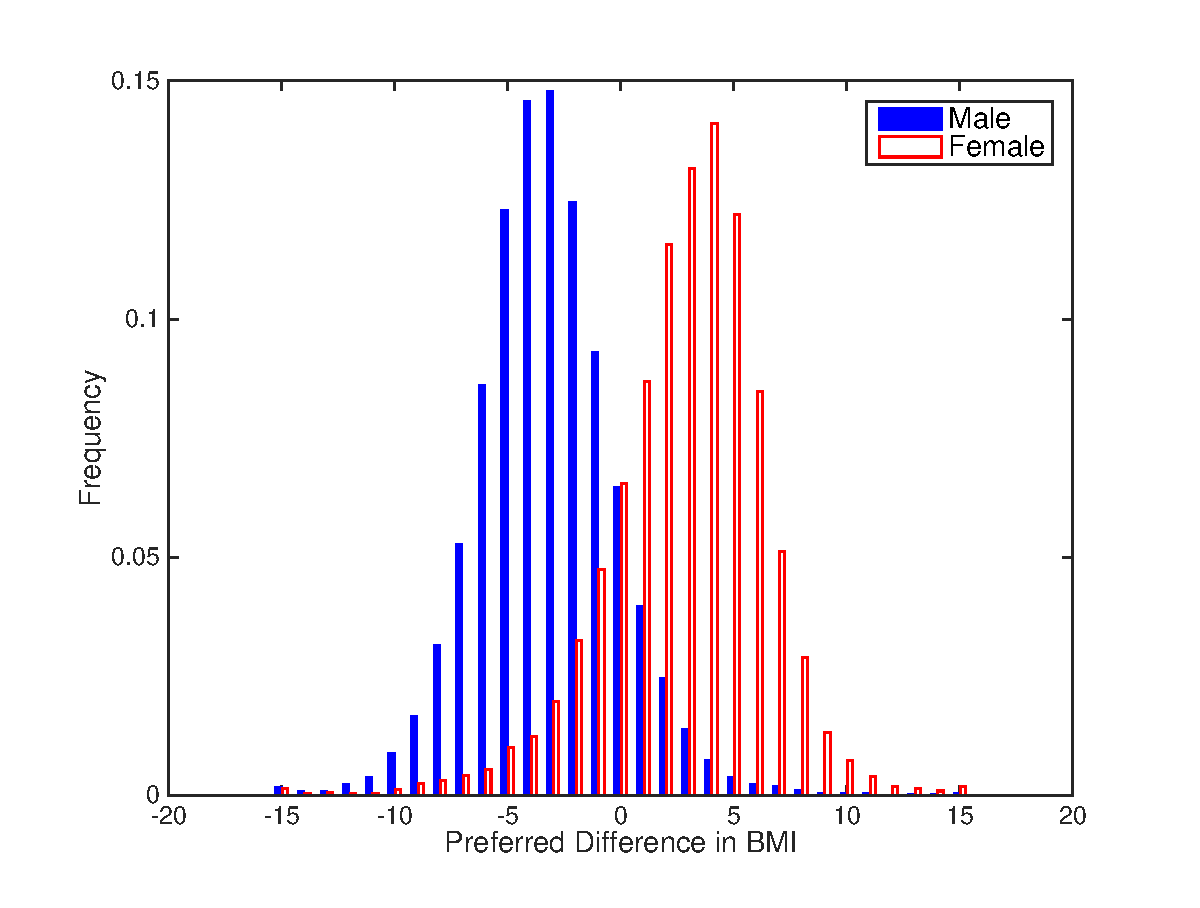
\includegraphics[scale=0.34]{imgDiff_BMI}
%		\label{fig:propertyDifferenceBMI}
%	}
%	\subfloat[Body Type]{
%		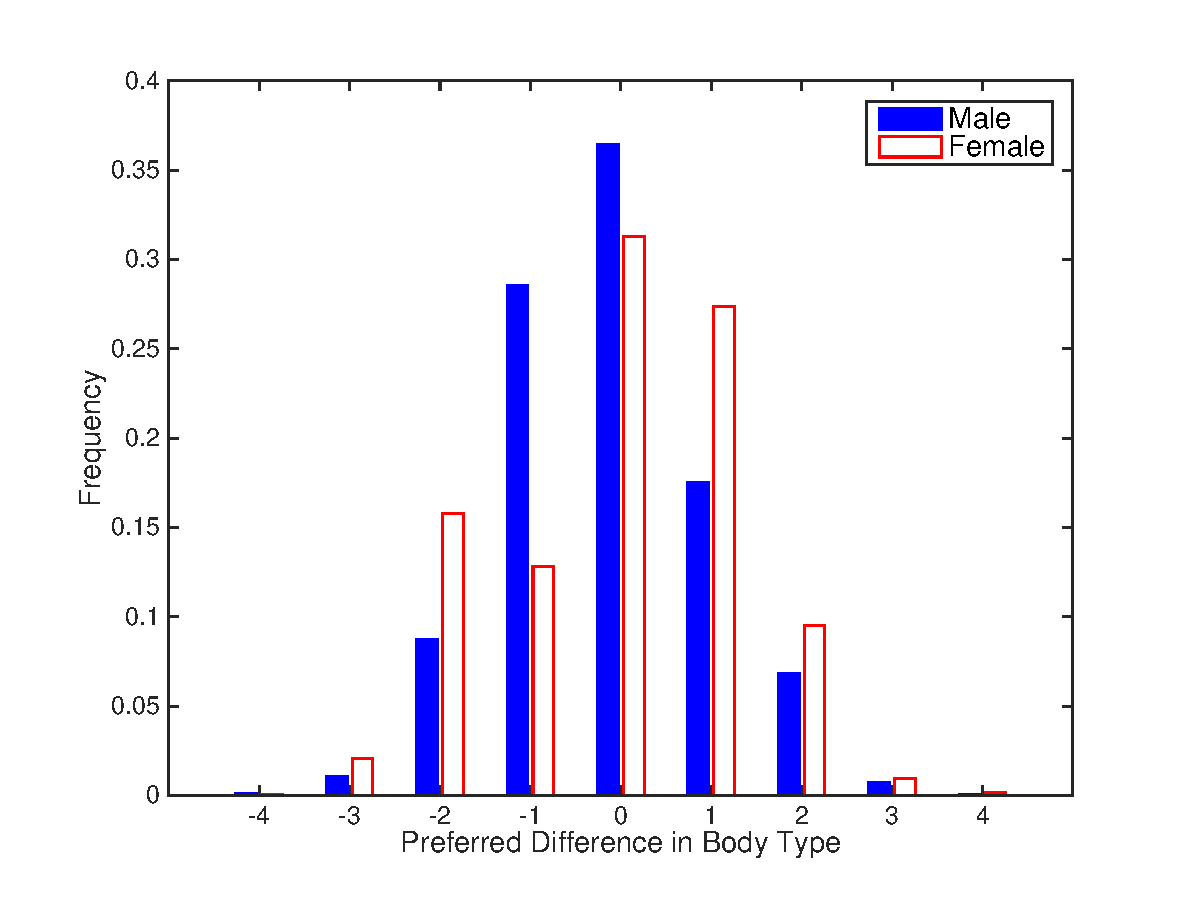
\includegraphics[scale=0.34]{imgDiff_BodyType}
%		\label{fig:propertyDifferenceBodyType}
%	} 
	\caption{
		Preferred difference distributions in 
		height, 
		age, 
		education, and
		income.
	}
	\label{fig:propertyDifference}
%\end{center}
\end{figure*}
%\end{figure}
% ------------------------------------------------------------------------
% =========================================================================




% =========================================================================
\subsection{Distributions of Preferred Differences}

Note that the average preferred differences of males and females are very close to each other in \reftbl{tbl:statistics}.
The standard deviations are also very close to each other.
If we assume that the male and female distributions are gaussian distributions,
the distributions should be very similar
as if female distribution is obtained by shifting the male distribution.
This cannot be a coincidence and deserves further study.
It seems males and females complement each other in the preferred differences.
Since we have not only the averages and standard deviations, 
but also the distributions,
we can further investigate the distributions for compatibility.

Distributions of preferred differences 
in age, education, and salary are given in 
\reffig{fig:propertyDifferenceAge},
\reffig{fig:propertyDifferenceEducation}, and
\reffig{fig:propertyDifferenceSalary}, respectively.
%Similar findings are observed 
%Besides homophily, 
%one observes that the average preferred differences of opposite genders 
%are in perfect harmony as seen in \reftbl{tbl:statistics}.
%Additional properties, namely body mass index and body type, given in \cite{Bingol2015si} are also in agreement. 
As we have deducted from \reftbl{tbl:statistics},
for all properties in \reffig{fig:propertyDifference},
the bell-shaped curves of male and female are also resemble to each other. 
One notices that
male curves are left-shifted, 
and female curves are right-shifted
with respect to the $y$-axis. 
%%This is also observed in \reftbl{tbl:statistics} 
%%as all male averages are negative and
%%female ones are positive.


%We interpret this, 
%as males prefer female with ``lower'' qualification. 
%Similarly females prefer male with ``higher'' qualifications.
%That is, 
%compared to themselves, 
%females prefer 
%taller and older males with 
%better education and higher income.

\hbIdea{compatible} % ====================
In order to get better understanding,
consider a simplified example given in \reffig{fig:propertyDifferenceDummy}.
% *****************
Note that
females that prefer $\Delta p = x$
matches with 
males that prefers $\Delta p = -x$.
Therefore,
we should not compare the distribution $f(x)$ of females
not with $m(x)$ of males as we previously thought.
We should compare $f(x)$ with $m(-x)$,
the symmetric graph with respect to the $y$-axis.
We make a reasonable assumption that 
there are equal number of men and women.
Then
$\min\{ {f(x), m(-x)} \}$ of the women who prefer $\Delta p = x$ are matched.
Then, 
the \emph{compatibility} of two distributions can be measured by means of the ratio of matched women given as
\[
	\rho = \sum_{x} \min\{ {f(x), m(-x)} \}
\]
where summation is taken over all possible values of $x$.
This is a well-defined metric since 
the ratio of matched women is equal to that of men.

In \reftbl{tbl:statistics}, 
the properties are listed in ascending order in compatibility.
Height is the property with the lowest compatibility.
Even for this case,
$90~\%$ of the population can find a satisfying partner.
Interestingly,
income has the highest compatibility and age comes next. 


% =========================================================================
% FIG HERE 
% {fig:propertyDifferenceDummy}
% ------------------------------------------------------------------------
\begin{figure}%[ht]
\centering
%\begin{center}
%	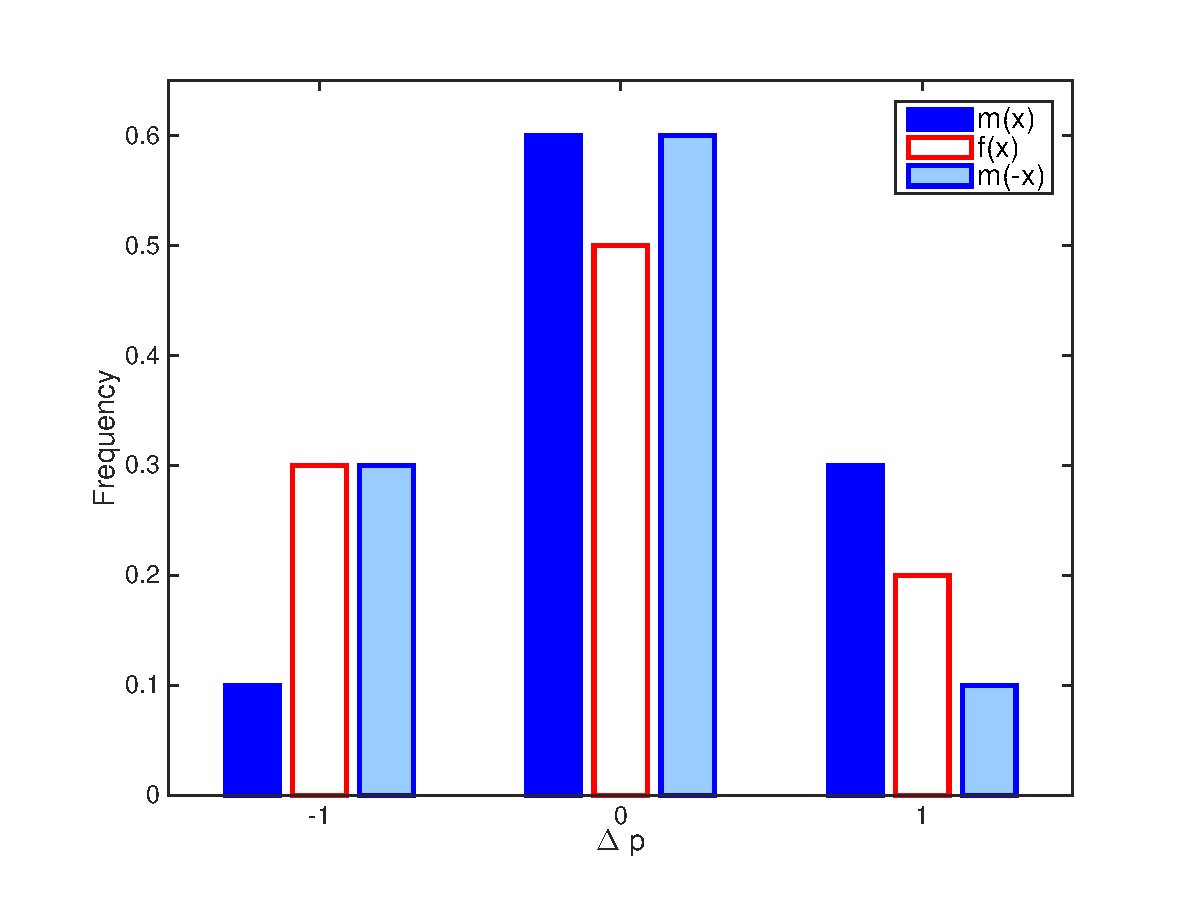
\includegraphics[width=.8\columnwidth]{imgDiff_Dummy}
	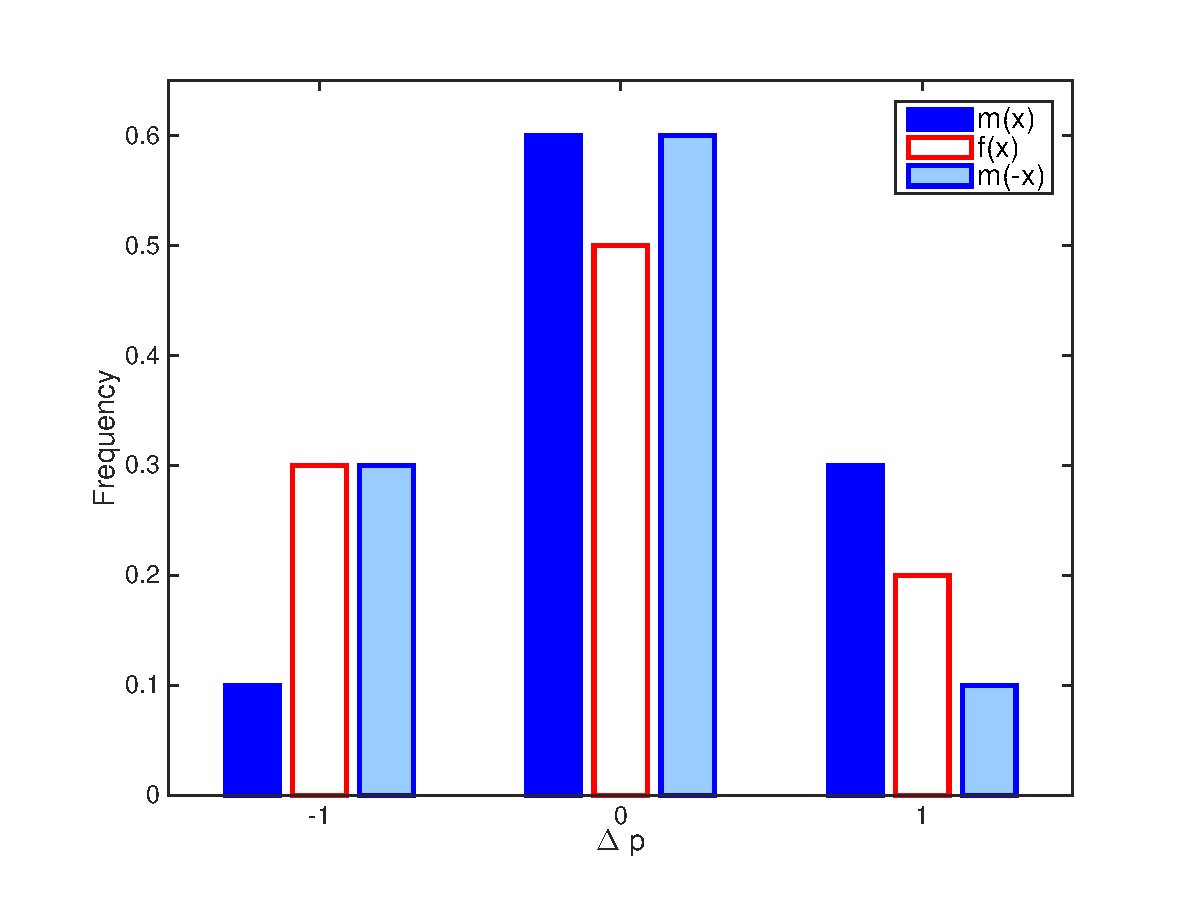
\includegraphics[width=\myFigWidth]{imgDiff_Dummy}
	\caption{
		Distribution of difference in 
		a dummy property $p$.
		We assume that male female populations are the same.
		%
		(i)~$50\%$ of women and 
		$60\%$ of men prefer no differences in $p$.
		Hence $50\%$ matches for $\Delta p = 0$.
		%
		(ii)~$20\%$ of women who prefer difference of $\Delta p = 1$ 
		are to match with
		$10\%$ of men who prefer differences of $\Delta p = -1$.
		Only $10\%$ matches for $\Delta p = 1$.
		%
		(iii)~$30\%$ of women who prefer difference of $\Delta p = -1$ 
		are exactly match with
		$30\%$ of men who prefer differences of $\Delta p = 1$.
		That is, $30\%$ matches for $\Delta p = 1$.
		%
		In total $90\%$ of women are match.
		Hence male female compatibility is $\rho = 0.90$.
	}
	\label{fig:propertyDifferenceDummy}
%\end{center}
\end{figure}
% ------------------------------------------------------------------------
% =========================================================================



% =========================================================================
\hbSection{Discussion}

\hbIdea{discussion} % ====================
In real life, 
men and women behave differently.
Our findings show that 
the virtual world of online dating is another manifestation of this difference.
%
(i)~While male prefers women with lower qualifications in every property 
that we have investigated, 
women just do the opposite. 
%
(ii)~Interestingly, the preferences of men and women match to each other so that 
the number of dissatisfied is minimized.
Due to lack of space, we do not report here but 
we have also observed similar findings in body mass index and body type, 
too~\cite{
	Bingol2012PartnerArxiv}. 
	
We can explain this evolutionary dynamic.
Suppose we start with individual with uniform one individual prefers difference far away from the
We are not in that position but 
it would be nice if we could provide explanations for these findings.
It may be possible to find some evolutionary 
explanation~\cite{
	Kenrick1992,
	Silverman1992,
	Pawlowski2000Nature}.

%We want to point out two more observations. 
%%
%(i)~The data clearly indicates that men take the first move in partner selection. 
%Then, women have the right to accept or reject. 
%%
%(ii)~On the average females make more partners than males,
%since there are 
%$29,274$ male and 
%$14,981$ female users to make partners,
%there is 1 female for 2 males.
%Note that this disagrees with 
%men having more sexual partners than women~\cite{
%	Liljeros2001Nature}.
%It might be the case that 
%this ratio changes 
%when it comes to physical relationship.



\hbIdea{warnings} % ====================
One needs to be careful on a number of issues in a study like that.
% 
(i)~One has to keep in mind that 
the findings could be culture dependent.
%
(ii)~The profile is based on user's claim, 
that is, 
it may be misleading. 
On the other hand, 
stretching the properties too far would not be a good strategy 
since unfaithful declaration, 
such as declared as slim while being obese, 
would be an obstacle to further the relationship
when the time comes to meet face-to-face~\cite{
	Norcie2013LNCS,
	Ellison2013}.
So we assume that users are closed to what they claim to be.
%
(iii)~Privacy is the most important issue for such an investigation.
In this study no data left the company. 
All the data processing is done at their site.
No individual personal information is used.
Only statistical data such as given in \reffig{fig:propertyDifference} is shared with us.

\section*{Acknowledgment}
This work was partially supported 
by Bogazici University Research Fund, BAP-2008-08A105, 
by the Turkish State Planning Organization (DPT) TAM Project, 2007K120610,
and
by COST action MP0801.








% An example of a floating figure using the graphicx package.
% Note that \label must occur AFTER (or within) \caption.
% For figures, \caption should occur after the \includegraphics.
% Note that IEEEtran v1.7 and later has special internal code that
% is designed to preserve the operation of \label within \caption
% even when the captionsoff option is in effect. However, because
% of issues like this, it may be the safest practice to put all your
% \label just after \caption rather than within \caption{}.
%
% Reminder: the "draftcls" or "draftclsnofoot", not "draft", class
% option should be used if it is desired that the figures are to be
% displayed while in draft mode.
%
%\begin{figure}[!t]
%\centering
%\includegraphics[width=2.5in]{myfigure}
% where an .eps filename suffix will be assumed under latex, 
% and a .pdf suffix will be assumed for pdflatex; or what has been declared
% via \DeclareGraphicsExtensions.
%\caption{Simulation results for the network.}
%\label{fig_sim}
%\end{figure}

% Note that the IEEE typically puts floats only at the top, even when this
% results in a large percentage of a column being occupied by floats.


% An example of a double column floating figure using two subfigures.
% (The subfig.sty package must be loaded for this to work.)
% The subfigure \label commands are set within each subfloat command,
% and the \label for the overall figure must come after \caption.
% \hfil is used as a separator to get equal spacing.
% Watch out that the combined width of all the subfigures on a 
% line do not exceed the text width or a line break will occur.
%
%\begin{figure*}[!t]
%\centering
%\subfloat[Case I]{\includegraphics[width=2.5in]{box}%
%\label{fig_first_case}}
%\hfil
%\subfloat[Case II]{\includegraphics[width=2.5in]{box}%
%\label{fig_second_case}}
%\caption{Simulation results for the network.}
%\label{fig_sim}
%\end{figure*}
%
% Note that often IEEE papers with subfigures do not employ subfigure
% captions (using the optional argument to \subfloat[]), but instead will
% reference/describe all of them (a), (b), etc., within the main caption.
% Be aware that for subfig.sty to generate the (a), (b), etc., subfigure
% labels, the optional argument to \subfloat must be present. If a
% subcaption is not desired, just leave its contents blank,
% e.g., \subfloat[].


% An example of a floating table. Note that, for IEEE style tables, the
% \caption command should come BEFORE the table and, given that table
% captions serve much like titles, are usually capitalized except for words
% such as a, an, and, as, at, but, by, for, in, nor, of, on, or, the, to
% and up, which are usually not capitalized unless they are the first or
% last word of the caption. Table text will default to \footnotesize as
% the IEEE normally uses this smaller font for tables.
% The \label must come after \caption as always.
%
%\begin{table}[!t]
%% increase table row spacing, adjust to taste
%\renewcommand{\arraystretch}{1.3}
% if using array.sty, it might be a good idea to tweak the value of
% \extrarowheight as needed to properly center the text within the cells
%\caption{An Example of a Table}
%\label{table_example}
%\centering
%% Some packages, such as MDW tools, offer better commands for making tables
%% than the plain LaTeX2e tabular which is used here.
%\begin{tabular}{|c||c|}
%\hline
%One & Two\\
%\hline
%Three & Four\\
%\hline
%\end{tabular}
%\end{table}


% Note that the IEEE does not put floats in the very first column
% - or typically anywhere on the first page for that matter. Also,
% in-text middle ("here") positioning is typically not used, but it
% is allowed and encouraged for Computer Society conferences (but
% not Computer Society journals). Most IEEE journals/conferences use
% top floats exclusively. 
% Note that, LaTeX2e, unlike IEEE journals/conferences, places
% footnotes above bottom floats. This can be corrected via the
% \fnbelowfloat command of the stfloats package.




\section{Conclusion}
The conclusion goes here.





% if have a single appendix:
%\appendix[Proof of the Zonklar Equations]
% or
%\appendix  % for no appendix heading
% do not use \section anymore after \appendix, only \section*
% is possibly needed

% use appendices with more than one appendix
% then use \section to start each appendix
% you must declare a \section before using any
% \subsection or using \label (\appendices by itself
% starts a section numbered zero.)
%


\appendices
\section{Proof of the First Zonklar Equation}
Appendix one text goes here.

% you can choose not to have a title for an appendix
% if you want by leaving the argument blank
\section{???}

\hbIdea{large data} % ====================
Investigation of mating preferences
on larger population in traditional ways,
such as one-to-one interviews, 
becomes prohibitively difficult.
Thanks to Internet,
very interesting data sets~\cite{
	Centola2010Science, 
	Rocha2010PNAS,
	Szell2010PNAS,
	Szell2013SR,
	Kramer2014PNAS} 
have become available including
data on online dating~\cite{
	Barraket2008JSociology,
	Bingol2012PartnerArxiv,
	Norcie2013LNCS,
	Zhao2014IS,
	Ellison2013}.
Compared to 
$N = 10,047$ 
of \refcite{Buss1989} 
and
$N = 17,637$ of \refcite{Schmitt2008},
which are very big numbers,
we will investigate mating patterns of a population of 
$N = 44,253$
based on
the data of an online dating site. 


% use section* for acknowledgment
\section*{Acknowledgment}


The authors would like to thank...


% Can use something like this to put references on a page
% by themselves when using endfloat and the captionsoff option.
\ifCLASSOPTIONcaptionsoff
  \newpage
\fi



% trigger a \newpage just before the given reference
% number - used to balance the columns on the last page
% adjust value as needed - may need to be readjusted if
% the document is modified later
%\IEEEtriggeratref{8}
% The "triggered" command can be changed if desired:
%\IEEEtriggercmd{\enlargethispage{-5in}}

% references section

% can use a bibliography generated by BibTeX as a .bbl file
% BibTeX documentation can be easily obtained at:
% http://mirror.ctan.org/biblio/bibtex/contrib/doc/
% The IEEEtran BibTeX style support page is at:
% http://www.michaelshell.org/tex/ieeetran/bibtex/
%\bibliographystyle{IEEEtran}
% argument is your BibTeX string definitions and bibliography database(s)
%\bibliography{IEEEabrv,../bib/paper}

%%% HB VVV for doi link
%%http://tex.stackexchange.com/questions/84133/hyperlink-each-bib-entry-to-its-doi-page
%\def\mybibdoicolor{\color{blue!75!black}} %change color to suit.
%\newcommand*{\doi}[1]{\href{http://dx.doi.org/\detokenize{#1} {\raggedright\mybibdoicolor{DOI: \detokenize{#1}}}}
%%% HB AAA for doi link

\IEEEtriggeratref{32}
\bibliographystyle{IEEEtran}
\bibliography{IEEEabrv,bingol-PaperTemplateIEEE}


%
%% <OR> manually copy in the resultant .bbl file
%% set second argument of \begin to the number of references
%% (used to reserve space for the reference number labels box)
%\begin{thebibliography}{1}
%
%\bibitem{IEEEhowto:kopka}
%H.~Kopka and P.~W. Daly, \emph{A Guide to \LaTeX}, 3rd~ed.\hskip 1em plus
%  0.5em minus 0.4em\relax Harlow, England: Addison-Wesley, 1999.
%
%\end{thebibliography}

% biography section
% 
% If you have an EPS/PDF photo (graphicx package needed) extra braces are
% needed around the contents of the optional argument to biography to prevent
% the LaTeX parser from getting confused when it sees the complicated
% \includegraphics command within an optional argument. (You could create
% your own custom macro containing the \includegraphics command to make things
% simpler here.)
%\begin{IEEEbiography}[{\includegraphics[width=1in,height=1.25in,clip,keepaspectratio]{mshell}}]{Michael Shell}
% or if you just want to reserve a space for a photo:

%\begin{IEEEbiography}{Haluk~O.~Bingol}
\begin{IEEEbiographynophoto}{Haluk~O.~Bingol}
	Assoc. Prof. 
	His research interests include 
	social systems, 
	complex systems, 
	and human brain.
	Ph.D. in Computer Engineering, Syracuse University.
	email:~bingol@boun.edu.tr.
\end{IEEEbiographynophoto}
%\end{IEEEbiography}

% if you will not have a photo at all:
\begin{IEEEbiographynophoto}{Omer~Basar}
	Software Manager.
	His research interests include 
	Machine Learning, 
	Artificial Intelligence, 
	Robotics.
	M.S. in Computer Engineering, Bogazici University.
	email:~omerbasar@gmail.com.	
\end{IEEEbiographynophoto}

% insert where needed to balance the two columns on the last page with
% biographies
%\newpage

% You can push biographies down or up by placing
% a \vfill before or after them. The appropriate
% use of \vfill depends on what kind of text is
% on the last page and whether or not the columns
% are being equalized.

%\vfill

% Can be used to pull up biographies so that the bottom of the last one
% is flush with the other column.
%\enlargethispage{-5in}



% that's all folks
\end{document}


